%\pdfminorversion=4
\documentclass[xcolor=dvipsnames,hyperref={pdfpagelabels=false},unknownkeysallowed]{beamer}
\usepackage{tabls}
\usepackage{picture}
\usepackage{graphicx}
\usepackage{subcaption}
\captionsetup{compatibility=false}
%\usepackage{animate}

%To add a grid to the slides for aligning stuff
%\usepackage[texcoord,grid,gridunit=mm,gridcolor=gray,subgridcolor=gray!10,gridBG=true]{eso-pic}



%Load the myriad packages
\usepackage{tikz}
\usetikzlibrary{shapes.geometric, arrows}
\tikzstyle{startstop} = [rectangle, rounded corners, minimum width=2cm, text
    width=1.8cm, minimum height=1cm,text centered, text=white,draw=black, fill=Gray!140]
\tikzstyle{io} = [trapezium, trapezium left angle=70, trapezium right angle=110,
minimum width=0.5cm, minimum height=1cm, text centered, draw=black,
fill=blue!20!Gray!90!,text=white]
\tikzstyle{process} = [rectangle, minimum width=2cm, minimum height=1cm, text
centered, text width=2cm, draw=black, text=white,fill=Gray!140!blue!70!white]
\tikzstyle{decision} = [diamond, minimum width=2.0cm, minimum
    height=0.81cm,aspect=1.40, text centered, draw=black, fill=Gray!,text=white]
\tikzstyle{arrow} = [thick,line width=0.5mm,->,>=stealth]
\tikzstyle{arrow1} = [dashed,->,>=stealth]

\usepackage[absolute,overlay]{textpos}

\newdimen\pc \pc=14bp
\def\XY#1#2{\xy{#1\pc}{#2\pc}}

\newcommand\myblock[3]{%
    \begin{textblock*}{\paperwidth}(#1\paperwidth,#2\paperwidth)
        \raggedright #3\hspace{0.5em}
    \end{textblock*}}


%\definecolor{myblue}{rgb}{0.7, 0.7, 60.0}
\definecolor{mylightblue}{rgb}{1,1,1}
\newcommand*{\boxedcolor}{blue}
\makeatletter
\renewcommand{\boxed}[1]{\textcolor{\boxedcolor}{%
  \fbox{\normalcolor\m@th$\displaystyle#1$}}}
\makeatother

\renewcommand{\u}[1]{\underline{#1}}

\newcommand{\iso}[2]{${}^{{#2}}${#1} }
\newcommand{\nubar}[0]{$\overline{\nu}$ }
\newcommand{\keff}[0]{\ensuremath{{k}_{\textsf{eff}}} }
\newcommand{\expect}[1]{E[#1] }
\newcommand{\colg}[1]{{\color{ForestGreen} #1}}
\newcommand{\coly}[1]{{\color{yellow} #1}}
\newcommand{\colb}[1]{{\color{blue} #1}}
\newcommand{\colG}[1]{{\color{Gray} #1}}
\newcommand{\colr}[1]{{\color{red} #1}}
\usepackage{amsfonts}
\newlength{\wideitemsep}
\setlength{\wideitemsep}{8pt}
\addtolength{\wideitemsep}{5pt}
\let\olditem\item
\renewcommand{\item}{\setlength{\itemsep}{\wideitemsep}\olditem}

\newcommand{\N}{\mathbb{N}}
\newcommand{\Z}{\mathbb{Z}}
\newcommand{\deriv}[2]{\frac{\mathrm{d} #1}{\mathrm{d} #2}}
\newcommand{\pderiv}[2]{\frac{\partial #1}{\partial #2}}
\newcommand{\bx}{\mathbf{X}}
\newcommand{\ba}{\mathbf{A}}
\newcommand{\by}{\mathbf{Y}}
\newcommand{\bj}{\mathbf{J}}
\newcommand{\bs}{\mathbf{s}}
\newcommand{\B}[1]{\ensuremath{\mathbf{#1}}}
\newcommand{\Dt}{\Delta t}
\renewcommand{\d}{\mathsf{d}}
\newcommand{\mom}[1]{\langle #1 \rangle}
\newcommand{\cur}[1]{\left\{ #1 \right\}}
\newcommand{\xl}{{x_{i-1/2}}}
\newcommand{\xr}{{x_{i+1/2}}}
\newcommand{\il}{{i-1/2}}
\newcommand{\ir}{{i+1/2}}
\newcommand{\shorttitle}{\color{black} A HOLO Algorithm for Thermal Radiative Transfer
    \makebox[\linewidth]{\rule{\textwidth}{5pt}}
}

%The next lines automatically add outline slides at start of each section
\AtBeginSection[]
{
    \begin{frame}<*>
        \frametitle{\shorttitle}
        \vspace{0pt}
        \begin{minipage}[c][0.6\textheight]{0.2\textwidth}
            \hspace{-2em}
\includegraphics[width=\textwidth]{tamu_seal.png}\hspace{1em}
            \rule[-0.3\textheight]{1pt}{0.8\textheight}
        \end{minipage}
    \vspace{0pt}
        \begin{minipage}[c][0.6\textheight]{0.74\textwidth}
        \tableofcontents[currentsection,currentsubsection]
         \end{minipage}
    \end{frame}
}

\setbeamerfont{frametitle}{size=\fontsize{13.7pt}{14.2pt}}
\setbeamerfont{normal font}{size=\tiny}

\graphicspath{{figures/}}

\usepackage{verbatim}
\usepackage{comment}
\usepackage[]{datetime}
\usepackage{multirow}
\newcommand{\thedate}{\today}

%Adjust margin to be more towards the right
\setlength\leftmargini{0.15\textwidth}
\addtolength\leftmarginii{0.05\textwidth}
\setbeamersize{sidebar width left=0.21em}
\setbeamersize{sidebar width right=0.21em}
\addtobeamertemplate{frametitle}{\vspace{0.31em}}{}

%\addtobeamertemplate{navigation symbols}{}{ %
%    \usebeamerfont{footline}%
%    \usebeamercolor[fg]{footline}%
%    \insertframenumber/\inserttotalframenumber
%}


% HACKING IN page numbers
%
%    \expandafter\def\expandafter\insertlogo\expandafter{%
%        \insertlogo\hspace{4pt}%
%        \raisebox{-6.9pt}{\scriptsize{\insertframenumber\,/\,\inserttotalframenumber}}}

\setlength{\tabcolsep}{1.05cm}

%Aggie-themed
\pgfdeclareimage[height=0.1in]{TAMUlogo}{tamu_engineering.png}
%\logo{\raisebox{-8pt}{\pgfuseimage{TAMUlogo}}}
\setlength\tabcolsep{0.2310in}
\titlegraphic{\centering\begin{tabular}{lcr}\hspace{-2em}
\includegraphics[trim=0.0in 0.0in 0.0in 0.0in,clip,height=0.18\textheight]{NEUP.jpg} &
 \hspace{-1em}
\includegraphics[height=0.18\textheight]{tamu_seal.png} &
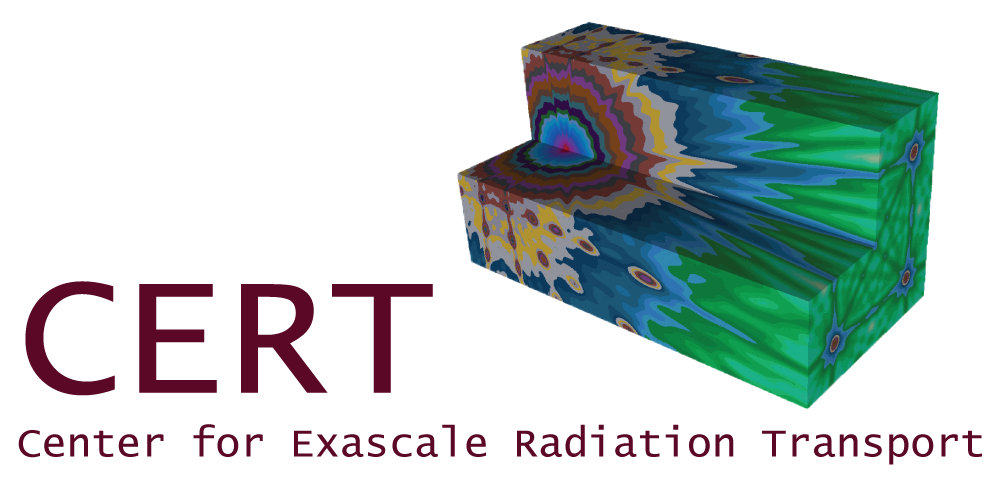
\includegraphics[height=0.18\textheight]{cert_logo_maroon.png}\end{tabular}}
%Michigan-themed
%\pgfdeclareimage[height=0.1in]{UMlogo}{michigan_engineering.png}
%\logo{\raisebox{-8pt}{\pgfuseimage{UMlogo}}}
%\titlegraphic{
\includegraphics[height=0.2\textheight]{michigan_block_m.png}}


%%%%%%%%%%%%%%%%%%%%%%%%%%%%%%%%%%%%%%%%%%%%%%%%%%%%%%%%%%%%%%%
% Optional packages, used to show off certain tricks

\newlength \figwidth
\setlength \figwidth {0.5\textwidth}


%%%%%%%%%%%%%%%%%%%%%%%%%%%%%%%%%%%%%%%%%%%%%%%%%%%%%%%%%%%%%%%

\usepackage[english]{babel}
\usetheme{boxes}

%Make it Aggie Maroon
\usecolortheme[RGB={80,0,0}]{structure}  
%Or Michigan Blue
%\usecolortheme[RGB={0,0,153}]{structure}  
%Or Michigan Maize
%\usecolortheme[RGB={255,204,0}]{structure}  


\setbeamertemplate{headline}{}
\setbeamertemplate{navigation symbols}{}%remove navigation symbols
\setbeamertemplate{footline}[frame number]



\setbeamersize{text margin left=1cm}
\setbeamersize{text margin right=1cm}

\makeatletter
\let\old@rule\@rule
\def\@rule[#1]#2#3{\textcolor{rulecolor}{\old@rule[#1]{#2}{#3}}}
\makeatother

\definecolor{rulecolor}{RGB}{80,0,0}


  % This will typeset only the frames (or slides) that have the given label ("current" in this case).

\title[HOLO for TRT]{A High-Order Low-Order Algorithm with Exponentially-Convergent Monte Carlo for
    Thermal Radiative Transfer}
    \author[S.R. Bolding]{{Simon Bolding \\ \vspace{1.0em}\emph{Preliminary Exam}}}
\date{{06 May 2016} }
\subject{}
%\institute{Los Alamos National Laboratory}

% \classificationlevel{SECRET/RD}
% \transmissible{}

%\reportnum{\textcolor{blue}{SAMPLE TEMPLATE ONLY \\ Contains NO Classified
%Information}}

% \dissableframenumber
\begin{document}
\setbeamercolor*{title}{use=structure,fg=white,bg=structure.fg}
\setbeamertemplate{title page}[default][colsep=-4bp,rounded=true,shadow=true]

\def\beginpage{\null\vfill\bgroup
\offinterlineskip\leftskip=\z@}
\def\endpage{\egroup\eject}

\begin{frame}
    \titlepage \vspace{-0.213in}
    \begin{center}
    \end{center}    
\end{frame}

\setlength{\tabcolsep}{6pt}

\setbeamercolor*{frametitle}{fg=Black!78}


%%%%%%%%%%%%%%%%%%%%%%%%%%%%%%%%%%%%%%%%%%%%%%%%%%%%%%%%%%%%%%%%%%%%%%%%%%%%%%%%%%%%%%%%%
\begin{frame}
\frametitle{We are interested in modeling thermal radiation transport \\ in the high energy,
    density physics regime.}
    \addtolength{\wideitemsep}{0.08in}
\begin{itemize}
    \item[] Materials under extreme conditions \\ \colG{Temperatures on order of $10^6$ K or more}
    \item[] Photon radiation field interacts with material \\ 
        \colG{Significant \colb{energy} and momentum may be exchanged}
 \item[] We want to improve efficiency of calculations \\
     \colG{for inertial confinement fusion, supernovae, et. al.}
    \end{itemize}
\end{frame}


%%%%%%%%%%%%%%%%%%%%%%%%%%%%%%%%%%%%%%%%%%%%%%%%%%%%%%%%%%%%%%%%%%%%%%%%%%%%%%%%%%%%%%%%%
\begin{frame}
\frametitle{Our method has been applied to a simplied model, \\ the 1D grey TRT equations}
\setlength{\unitlength}{\textwidth}
\begin{center}
\begin{align*}\label{ho_cont}
    \frac{1}{c}\pderiv{I}{t} + \mu \pderiv{I}{x} + \sigma_t I(x,\mu,t)
    &= \frac{1}{4\pi} \left( \sigma_a a c T^4 + \sigma_s \phi\right),
  \\
  C_v \pderiv{T(x,t)}{t} &=  \sigma_a \phi(x,t) - \sigma_a a c T^4\\
\end{align*}
\end{center}
\begin{itemize}
        \item Fundamental unknowns are the radiation intensity $I(x,\mu,t)$ and material
            temperature $T(x,t)$
        \item Equations are nonlinear and may be tightly coupled \\  
               \colG{through absorption and reemission of photons}
        \item For practical applications, spatial discretization must preserve the \colb{equilibrium diffusion limit} (EDL)
\end{itemize}
\end{frame}

%%%%%%%%%%%%%%%%%%%%%%%%%%%%%%%%%%%%%%%%%%%%%%%%%%%%%%%%%%%%%%%%%%%%%%%%%%%%%%%%%%%%%%%%%
\begin{frame}
\frametitle{Implicit Monte Carlo (IMC) is the standard Monte Carlo solution method for TRT problems.}
\begin{itemize}
\item[] The system is linearized over a time step \vspace{0.1in}
\setlength\wideitemsep{0.2in}
    \begin{itemize}
        \item Results in a \textbf{linear transport equation }
               \\ \colG{with effective emission and scattering terms}
\item Continuous time integration of intensity via MC
        \\ \colG{but opacities are evaluated at begining time and \emph{emission source is not fully implicit}}
        \item Use source tilting to mitigate energy propagation \\
            \colG{reconstruction of linear-discontinuous source shape}
    \end{itemize}
\end{itemize}
\end{frame}

\begin{frame}
    \frametitle{Our high-order low-order (HOLO) method improves several drawbacks of IMC}
{\scriptsize
\begin{tabular}{lr} \hline
\multicolumn{1}{c}{\textbf{IMC}} & \multicolumn{1}{c}{\colb{HOLO Method}} \\  \hline
Effective scattering cross section can be very large & LO system resolves nonlinearities \\
Linearization can cause non-physical results & Fully implicit time-discretization \\
\parbox{0.4\textwidth}{Reconstruction of linear source shape,\\ for preserving equilibrium diffusion limit} & Linear-discontinuous FE for $T(x)$
\end{tabular}
}
\end{frame}

\begin{frame}<*>
    \frametitle{\shorttitle}
        \vspace{0pt}
        \begin{minipage}[c][0.6\textheight]{0.2\textwidth}
            \hspace{-2em}
\includegraphics[width=\textwidth]{tamu_seal.png}\hspace{1em}
            \rule[-0.3\textheight]{1pt}{0.8\textheight}
        \end{minipage}
    \vspace{0pt}
        \begin{minipage}[c][0.6\textheight]{0.74\textwidth}
\tableofcontents[
hideothersubsections,
sectionstyle=show,
subsectionstyle=hide
]
         \end{minipage}
\end{frame}
%%%%%%%%%%%%%%%%%%%%%%%%%%%%%%%%%%%%%%%%%%%%%%%%%%%%%%%%%%%%%%%%%%%%%%%%%%%%%%%%%%%%%%%%%
\section{Overview of algorithm}

%%%%%%%%%%%%%%%%%%%%%%%%%%%%%%%%%%%%%%%%%%%%%%%%%%%%%%%%%%%%%%%%%%%%%%%%%%%%%%%%%%%%%%%%%
\begin{frame}
    \frametitle{We solves a non-linear low-order system with high-order angular correction from efficient MC simulations.}
    \setlength{\unitlength}{1mm}
    \begin{picture}(120,80)(0,-80)
    \put(-5,-15){
    \begin{minipage}[t]{1.1\textwidth}
        \begin{itemize}
\setlength\wideitemsep{0.06in}
            \item[] The \textbf{LO system} consists of space-angle moment equations,\\
                    \colG{formed over a fixed finite-element (FE) spatial mesh}
                \vspace{0.02in}
                {\scriptsize
                \begin{itemize}
                    \item Reduced dimensionality in angle\\
                         \colG{allows for solution with Newton's method}
              \item \textbf{Output:} a linear-discontinuous (LD) FE representation
                        of \colb{scattering and emission source}
                  %  \item Consistency terms derived directly from transport equation
                \end{itemize}
}\vspace{0.04in}
            \item[] The \textbf{HO system} is pure-absorber transport problem
                {\scriptsize
                \begin{itemize}
                    \item Solved with exponentially-convergent MC (ECMC) \\ \colG{for efficient reduction of statistical noise }
                    \item \textbf{Output:} \colb{angular consistency terms}
                \end{itemize}
}
        \end{itemize}
    \end{minipage}

}
\end{picture}
\end{frame}


\begin{frame}
    \frametitle{Iterations between the HO and LO systems \\ are performed each time step}
    %\fontsize{9}{5.0}\selectfont
        \hspace{-0.1in}
        \resizebox{1.04\linewidth}{!}{
    \fontsize{10}{12.0}\selectfont
    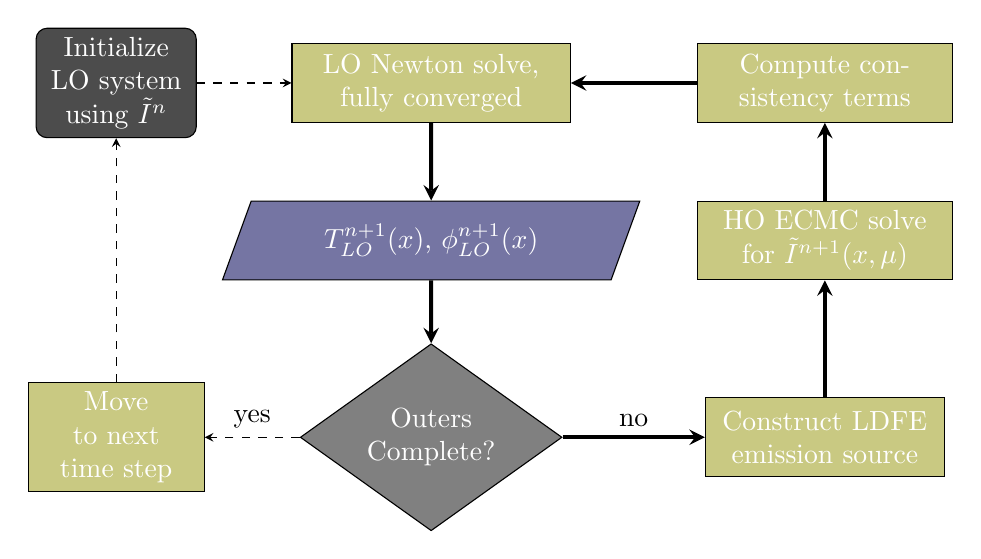
\begin{tikzpicture}[node distance=2cm]
        \node (start) [startstop] {Initialize LO system using $\tilde{I}^n$};
        \node (in1) [process, right of=start, xshift=2cm, text width=3.3cm]  {
        {LO Newton solve, fully converged}};
        \node (pro1) [io, below of=in1] {$T_{LO}^{n+1}(x)$, $\phi_{LO}^{n+1}(x)$};
        \node (dec1) [decision, below of=pro1, yshift=-0.5cm, text width=1.74cm] {Outers Complete?};
        \node (pro2a) [process, left of=dec1, xshift=-2.0cm] {Move to next time
        step};
        \node (srcs) [process, right of=dec1, xshift=3.0cm, text width=2.8cm] {
        {Construct LDFE emission source}};
        \node (pro2b) [process, text width=3.0cm, above of=srcs, yshift=0.5cm] {{HO ECMC solve}
           for $\tilde I^{n+1}(x,\mu)$};
        \node (cons) [process, above of=pro2b, text width=3.0cm] {{Compute consistency
        terms}};
        \draw [arrow1] (start) -- (in1);
        \draw [arrow] (in1) -- (pro1);
        \draw [arrow] (pro1) -- (dec1);
        \draw [arrow] (srcs) -- (pro2b);
        \draw [arrow] (dec1.east) -- node[anchor=south] {no} (srcs);
        \draw [arrow1] (dec1.west) -- node[anchor=south] {yes} (pro2a);
        \draw [arrow1] (pro2a) -- (start);
        \draw [arrow] (pro2b) -- (cons);
        \draw [arrow] (cons) -- (in1);
    \end{tikzpicture}
}
\end{frame}


%%%%%%%%%%%%%%%%%%%%%%%%%%%%%%%%%%%%%%%%%%%%%%%%%%%%%%%%%%%%%%%%%%%%%%%%%%%%%%%%%%%%%%%%%
%\begin{frame}
%    \frametitle{High-Order Low-Order Algorithm}
%    %\fontsize{9}{5.0}\selectfont
%        \resizebox{0.99\linewidth}{!}{
%    \fontsize{10}{12.0}\selectfont
%    \begin{tikzpicture}[node distance=2cm]
%        \node (start) [startstop] {Initialize LO system using ${I}^n$};
%        \node (in1) [process, right of=start, xshift=2cm, text width=3.3cm]  {
%        {LO Newton solve, fully converged}};%{LO solve:\vspace{0.041in}        $\B D(\mu^{HO})\Phi = \frac{1}{\keff}\B F\Phi$};
%        \node (pro1) [io, below of=in1] {$T_{LO}^{n+1}(x)$, $\phi_{LO}^{n+1}(x)$};
%        \node (dec1) [decision, below of=pro1, yshift=-0.5cm, text width=1.74cm] {Outers Complete?};
%        \node (pro2a) [process, left of=dec1, xshift=-2.0cm] {Move to next time
%         step};
%        \node (srcs) [process, right of=dec1, xshift=3.0cm, text width=2.8cm] {
%        {Construct LD sources}};
%        \node (pro2b) [process, above of=srcs, yshift=0.5cm] {{HO ECMC Solve}};
%        \node (cons) [process, above of=pro2b, text width=3.0cm] {{Compute consistency
%        terms}};
%        \draw [arrow1] (start) -- (in1);
%        \draw [arrow] (in1) -- (pro1);
%        \draw [arrow] (pro1) -- (dec1);
%        \draw [arrow] (srcs) -- (pro2b);
%        \draw [arrow] (dec1.east) -- node[anchor=south] {no} (srcs);
%        \draw [arrow1] (dec1.west) -- node[anchor=south] {yes} (pro2a);
%        \draw [arrow1] (pro2a) -- (start);
%        \draw [arrow] (pro2b) -- (cons);
%        \draw [arrow] (cons) -- (in1);
%    \end{tikzpicture}
%}
%\end{frame}





\section{The LO system}
\subsection{}


%%%%%%%%%%%%%%%%%%%%%%%%%%%%%%%%%%%%%%%%%%%%%%%%%%%%%%%%%%%%%%%%%%%%%%%%%%%%%%%%%%%%%%%%%
\begin{frame}
    \frametitle{The LO equations are formed from spatial and angular moments of the TRT equations}
    \begin{itemize}
        \item A backward Euler time discretization is used\\ \colG{in both the HO and LO equations}
\item \colb{Linear discontinuous} FE in space for $\phi$, $T$, and $T^4(x)$   \end{itemize}
    \begin{centering}
        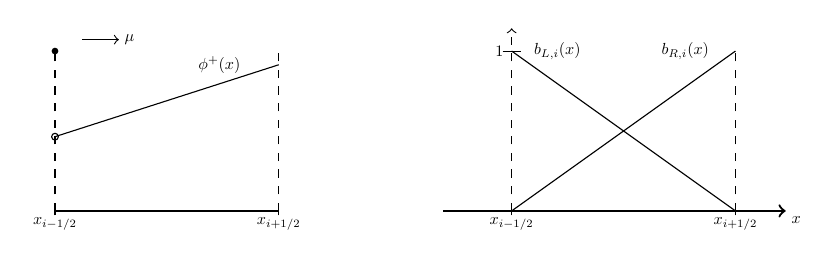
\begin{tikzpicture}[scale=0.58, every node/.style={transform shape}]
            \draw (1.0,4.0) node[fill,circle,inner sep=0pt,minimum
            size=4.2pt] {};
            \filldraw[color=black, fill=white] (1,2.1250) circle (2.1pt);
            \draw [->] (1.6,4.25) -- (2.4,4.25) node[anchor=west] {$\mu$};
            \draw (1.0,0.4) -- (1.0,0.6) node[below, pos=0.4] {$x_{i-1/2}$};
            \draw (5.90,0.4) -- (5.90,0.6) node[below, pos=0.4] {$x_{i+1/2}$};
            \node at (4.6,3.70) {$\phi^+(x)$};
            \draw [thick] (1.0,0.5) -- (5.9,0.5) node[anchor=north west] {};
            \draw (1.0,2.125) -- (5.90,3.70);
            \draw [dashed] (5.90,0.5) -- (5.90,4);
            \draw [dashed] (1.0,0.5) -- (1.0,4);

            \draw (10.8,4.0) -- (11.2,4.0) node[anchor=east]{$1$ \hspace{0.4em} };
            \draw (11.0,0.4) -- (11.0,0.6) node[below, pos=0.4] {$x_{i-1/2}$};
            \draw (15.90,0.4) -- (15.90,0.6) node[below, pos=0.4] {$x_{i+1/2}$};
            \node at (14.8,4.0) {$b_{R,i}(x)$};
            \node at (12.0,4.0) {$b_{L,i}(x)$};
            \draw [thick,->] (9.5,0.5) -- (17.0,0.5) node[anchor=north west] {$x$};
            \draw [dashed,-] (15.90,0.5) -- (15.90,4);
            \draw [dashed,->] (11.0,0.5) -- (11.0,4.5);
            \draw (11.0,0.5) -- (15.90,4.0);
            \draw (15.90,0.5) -- (11.0,4.0);
        \end{tikzpicture}
    \end{centering}
    \begin{itemize}
    \item \colb{Half-range integrals} over $+$ and $-$ $\mu$
    \item \emph{\u{Examples}} of moments:\vspace{-0.05in}
    \end{itemize}
    \begin{center}
    \begin{tabular}{cc}
        \underline{Spatial: left basis} & \underline{Angular: positive flow} \\ 
        $ {\displaystyle \mom{\cdot}_{L,i} = \frac{2}{h_i} \int_{x_\il}^{x_\ir}
        b_{L,i}(x)(\cdot) \d x \quad }$  & ${ \quad \displaystyle \phi^+(x) =
        2\pi\int_0^1 I(x,\mu) \d \mu}$
    \end{tabular}
    \end{center}
\end{frame}


%%%%%%%%%%%%%%%%%%%%%%%%%%%%%%%%%%%%%%%%%%%%%%%%%%%%%%%%%%%%%%%%%%%%%%%%%%%%%%%%%%%%%%%%%
\begin{frame}
    \frametitle{Forming the LO System}
    \vspace{-0.1in}
    {\small
    \begin{enumerate}
     %\item Take the FE spatial moments of the TRT equations over spatial elements.
     %   \item Integrate resulting transport equation over $+$ and $-$ $\mu$ half ranges 
      \item Applying moments to the TRT equations yields 4 radiation equations, and 2 material energy
          equations, per cell \vspace{-0.062in}
    \item The resulting radiation equations are  manipulated to produce weighted
        averages, which we refer to as \colb{consistency
          terms}, e.g.,
    \begin{equation*}
\{{\mu}\}_{L,i}^{+} := \frac{\displaystyle 
    \int\limits_0^1 \int\limits_\xl^\xr \mu \, b_{L,i}(x) 
I^{n+1}(x,\mu) \;\d x \d \mu } 
{\displaystyle \int\limits_0^1 \int\limits_\xl^\xr \, b_{L,i}(x)
I^{n+1}(x,\mu)\; \d x \d \mu} 
    \end{equation*}
    \vspace{-0.1in}
\item Use \colb{$\tilde{I}_{HO}^{n+1}(x,\mu)$} \& LD spatial closure to close the system
    \end{enumerate}
    \begin{itemize}
            
        \item Cell unknowns are: $\mom{\phi}_{L,i}^{+}$, $\mom{\phi}_{R,i}^{+}$,
        $\mom{\phi}_{L,i}^{-}$, $\mom{\phi}_{R,i}^{-}$, $T_{L,i}$, $T_{R,i}$
     \item Non-linear, fully discrete system, solved with approximate Newton's method
 \end{itemize}


}
\end{frame}



\section{Exponentially Convergent MC High-Order Solver}
\subsection{}



%%%%%%%%%%%%%%%%%%%%%%%%%%%%%%%%%%%%%%%%%%%%%%%%%%%%%%%%%%%%%%%%%%%%%%%%%%%%%%%%%%%%%%%%%
\begin{frame}
    \frametitle{Overview of Exponentially Convergent Monte Carlo}
    \begin{itemize}
        \item Each batch tallies the \colb{error} in current estimate of solution
            \begin{itemize}
    \item Can reduce statistical error \colb{globally} $\propto e^{-\alpha N}$
    \item In TRT problems, $I^{n}$ often provides a \emph{very good} approximation of
        $I^{n+1}$, significantly reducing the required number of histories
\end{itemize}
     \end{itemize}
    \begin{minipage}{0.6\linewidth}
        \vspace{-2.0in}
        
     \begin{itemize}
     \item Requires a \colr{functional form} of the angular intensity $\tilde I(x,\mu)$
            \begin{itemize}
                \item Use LD \u{\colb{projection}} of the solution onto a space-angle FE
                    mesh
        \item LD FE $\tilde  I^{HO}(x,\mu)$ allows for direct computation of
            consistency terms
    \end{itemize}
    \end{itemize}
    \end{minipage}
    \begin{minipage}[t]{0.3\linewidth}
        \centering
        \scalebox{0.8}{
        \begin{tikzpicture}
            \draw (1,1) rectangle (4,4);
            \node[draw,circle,inner sep=1.2 pt,fill] at (2.5,2.5) {};
            \node[above] at (2.5,2.5) {$(x_i,\mu_j)$};
            \draw (1.0,0.4) -- (1.0,0.6) node[below, pos=0.4] {$x_{i-1/2}$};
            \draw (4.0,0.4) -- (4.0,0.6) node[below, pos=0.4] {$x_{i+1/2}$};
            \draw (0.4,1.0) -- (0.6,1.0) node[left, pos=0.4] {$\mu_{j-1/2}$};
            \draw (0.4,4.0) -- (0.6,4.0) node[left, pos=0.4] {$\mu_{j+1/2}$};
            \draw [thick,->] (0.5,0.5) -- (5,0.5) node[anchor=north west] {$x$};
            \draw [thick,->] (0.5,0.5) -- (0.5,5) node[anchor=east] {$\mu$};
        \end{tikzpicture}
    }
    \end{minipage}%
\end{frame}


%%%%%%%%%%%%%%%%%%%%%%%%%%%%%%%%%%%%%%%%%%%%%%%%%%%%%%%%%%%%%%%%%%%%%%%%%%%%%%%%%%%%%%%%%
\begin{frame}
    \frametitle{High Order System and ECMC Algorithm}
        \begin{align*}
            \hspace{-0.2in}
            \left[\mu \pderiv{}{x} + \left(\sigma_t^{n+1}+\frac{1}{c\Delta t}\right)\right]I^{n+1}
            &= \frac{I^{n}}{c\Delta t} + \boxed{\frac{1}{4\pi}\left(\sigma_a^{n+1} a c
    T_{LO}^{n+1,4}+\sigma_s\phi_{LO}^{n+1}\right)} \\
            \B L I^{n+1} &= \colb{q_{LO}}
     \end{align*}
    \begin{itemize}
        \item \colb{Pure absorber} transport problem because we have LD
            representation of $T^4$ from LO solution
        \vspace{-0.3in}
        
        \end{itemize}
        \begin{block}{For each batch $m$:}
         \begin{itemize}
        \item Residual Equation: $\displaystyle \B L \tilde 
            \epsilon^{(m)} =
            \tilde r^{(m)} = q - \B L \tilde I^{n+1,(m)}$
        \item Compute $\tilde{\epsilon}^{(m)} = \B L^{-1} \tilde{r}^{(m)}$ with MC 
            \begin{itemize}
                \item Particles are allowed to stream along path $s$, $w(s)=w_0 e^{-\sigma_t s}$
                \item Use cell-wise {systematic} sampling for $|r^{(m)}|$ source
            \end{itemize}
        \item Update: $\tilde I^{n+1,(m)} = \tilde I^{n+1,(m-1)} + \tilde \epsilon^{(m)}$
        \begin{itemize}
            \item If $\tilde{\epsilon}$ is reduced each batch, \colb{exponential convergence
                achieved}
        \end{itemize}
    \end{itemize}
\end{block}
\end{frame}




\section{Computational Results}
\subsection{}

\begin{frame}
    \frametitle{Relevant Problem and Implementation Specifics }
    \begin{itemize}
    \item Difficulties in resolving the solution near the wave-front
        \begin{itemize}
            \item The LD representation of $I(x,\mu)$ results in negative values within a
                cell
            \item In these results, no correction is applied to the HO solution, and the LO
                solution uses lumped LD and S$_2$ equivalent terms in bad cells
        \end{itemize}
     
 \item \u{For all results}
        \begin{itemize}
    \item LO Newton iterations are is fully converged each solve
    \item Fixed $\Delta t$ of $0.001$ shakes (0.01 ns)
    \item One HO solve per time step (predictor-corrector)
        \begin{itemize}
            \item \emph{each HO} solve has 3 ECMC batches
        \end{itemize}
    \item $\sigma_s = 0$
    \end{itemize}
    \end{itemize}
\end{frame}

{
\setbeamertemplate{footline}{}
%%%%%%%%%%%%%%%%%%%%%%%%%%%%%%%%%%%%%%%%%%%%%%%%%%%%%%%%%%%%%%%%%%%%%%%%%%%%%%%%%%%%%%%%%
\begin{frame}
    \frametitle{Marshak Wave Test Problem}
    \centering
    \begin{block}{}
        \begin{itemize}
                {\footnotesize
            \item From equilibrium, a radiation source is applied at the left
                boundary at $t=0$. With $\sigma_a\propto T^{-3}$; energy slowly moves across the
                system.
            \item Transient solution after 5 shakes plotted as $T_r =
                \sqrt[4]{\phi/ac}$, with 200~$x$ and 4~$\mu$  cells }
        \end{itemize}
    \end{block}
    \begin{figure}
    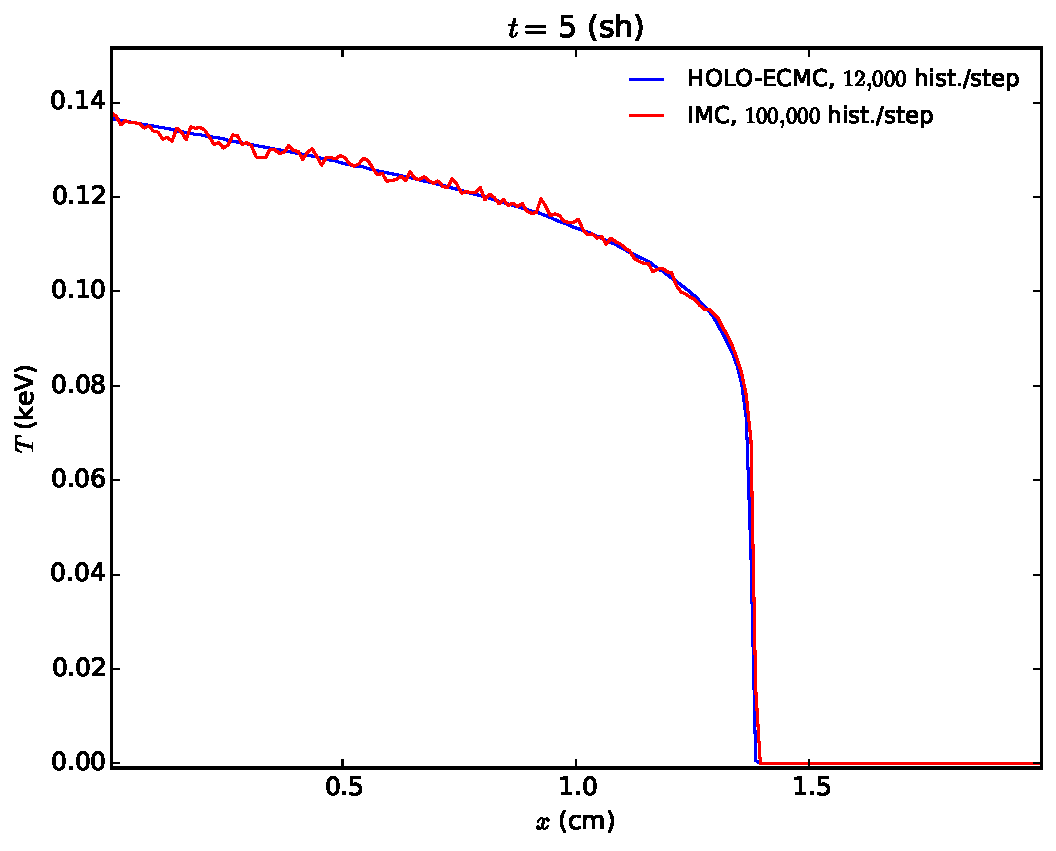
\includegraphics[width=0.615799\textwidth]{marshak_200_compare.pdf}
    \end{figure}
\end{frame}

%%%%%%%%%%%%%%%%%%%%%%%%%%%%%%%%%%%%%%%%%%%%%%%%%%%%%%%%%%%%%%%%%%%%%%%%%%%%%%%%%%%%%%%%%
\begin{frame}
    \frametitle{Two Material Problem, Comparison of Spatial Convergence}
    \begin{block}{}
        \begin{itemize}
            \item Same as Marshak Wave, but with constant opacities and an optically thin (left) and
                optically thick (right) region. ECMC uses 8 $\mu$ cells
        \end{itemize}
    \end{block}
\begin{figure}
    \centering
    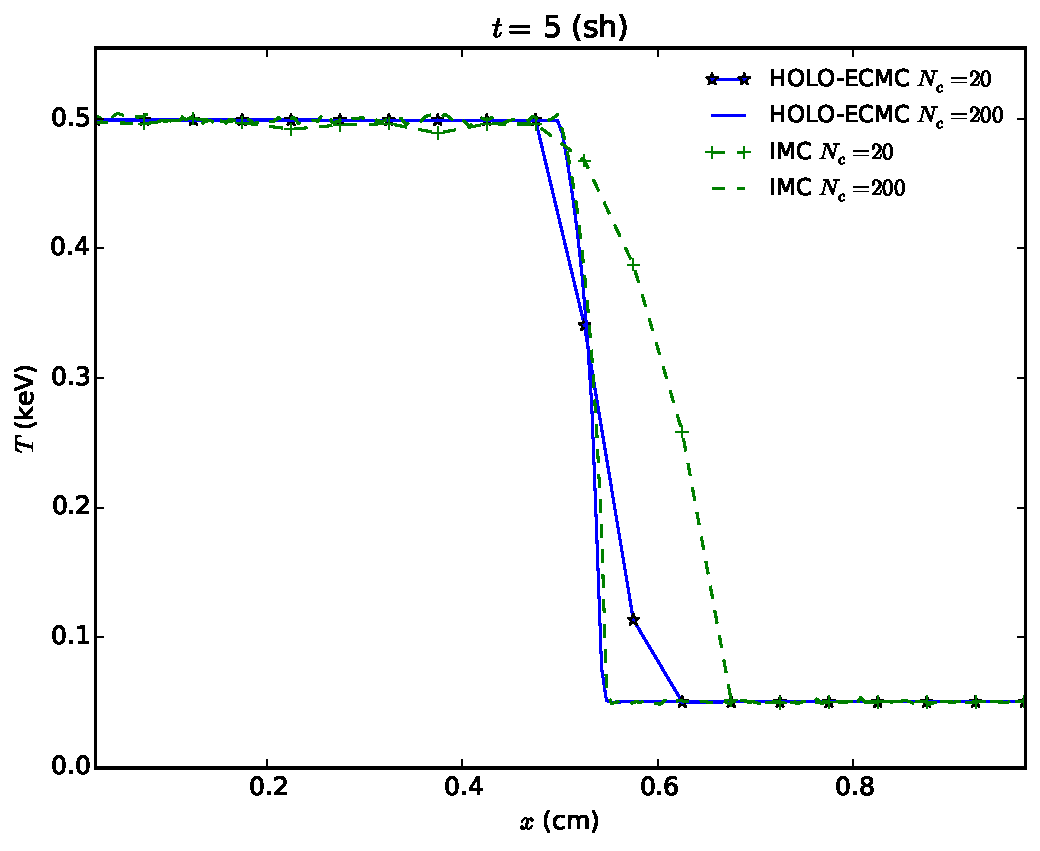
\includegraphics[width=0.6755799\textwidth]{two_mat_conv.pdf}
\end{figure}

\end{frame}


\begin{frame}
    \frametitle{DIFFUSION LIMIT PROBLEM}

\end{frame}

\begin{frame}
    \frametitle{Comparison of statistical noise for standard and ECMC HO solvers}
    \begin{block}{}
        {\small
    \begin{itemize}
        \item Different HO solvers: a
            comparison of
            \colb{ECMC} with 3 batches and standard MC (\colr{SMC}), as well as an S$_2$
            solution
    \end{itemize}
}
    \end{block}
    \centering
    \begin{figure}
    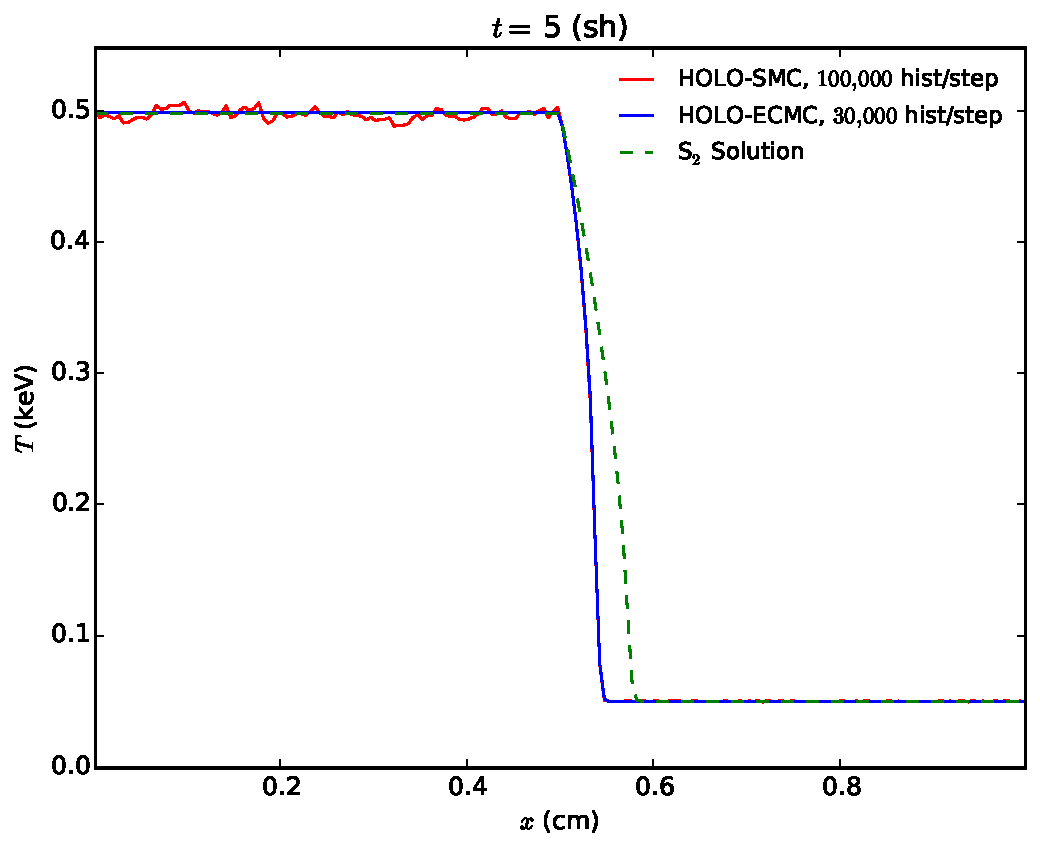
\includegraphics[width=0.6699\textwidth]{two_mat_ho_compare.pdf}
    \centering
    \end{figure}
\end{frame}

\begin{frame}
    \frametitle{ADD FOM AND ERROR FOR SMOOTH PROBLEM}

\end{frame}


}

%%%%%%%%%%%%%%%%%%%%%%%%%%%%%%%%%%%%%%%%%%%%%%%%%%%%%%%%%%%%%%%%%%%%%%%%%%%%%%%%%%%%%%%%%
\begin{frame}
    \frametitle{Current \& Future Development}
    \begin{itemize}
        \item Can accurately reproduce IMC results with HOLO method
        \begin{itemize}
            \item ECMC requires \colb{significantly less particles} than standard MC
            \item HO solver requires no effective scattering events
            \item LO solver determines non-linear Material temperature distribution
            \item LD representation of $T^4$ mitigates teleportation error
        \end{itemize}
        
    \item Currently developing strategies for dealing with unresolvable solutions
    \item Next step will be to implement in 2 spatial dimensions
    \end{itemize}
\end{frame}

\section{Remaining Research}
\begin{frame}
    \frametitle{We need a way to resolve issues when the LDFE projection produces non-physical solutions}
\end{frame}

\begin{frame}
    \frametitle{DSA with source iterations may provide a practical application of the LO equaitons in 2D}

\end{frame}

\begin{frame}
    \frametitle{We would like to use the HO solution to close the system}

\end{frame}


\begin{frame}
    \frametitle{\colb{There are several investigations left to do:}}
        \begin{enumerate}
            \item DSA
            \item hey
        \end{enumerate}
    \end{frame}

\date{}
\begin{frame}
    \frametitle{{\LARGE\coly{Questions?}}}
    \vspace{-0.21in}
    \titlepage \vspace{-0.2113in}
\end{frame}

\appendix
\newcounter{finalframe}
\setcounter{finalframe}{\value{framenumber}}

\title{Backup Slides}
\author{}
\date{}

%%%%%%%%%%%%%%%%%%%%%%%%%%%%%%%%%%%%%%%%%%%%%%%%%%%%%%%%%%%%%%%%%%%%%%%%%%%%%%%%%%%%%%%%%
\begin{frame}
    \frametitle{Two Material Problem, comparison in optically thin region}
    \begin{block}{}
        \begin{itemize}
            \item Plot of radiation temperature after 10 time steps
        \end{itemize}
    \end{block}
\begin{figure}
    \centering
    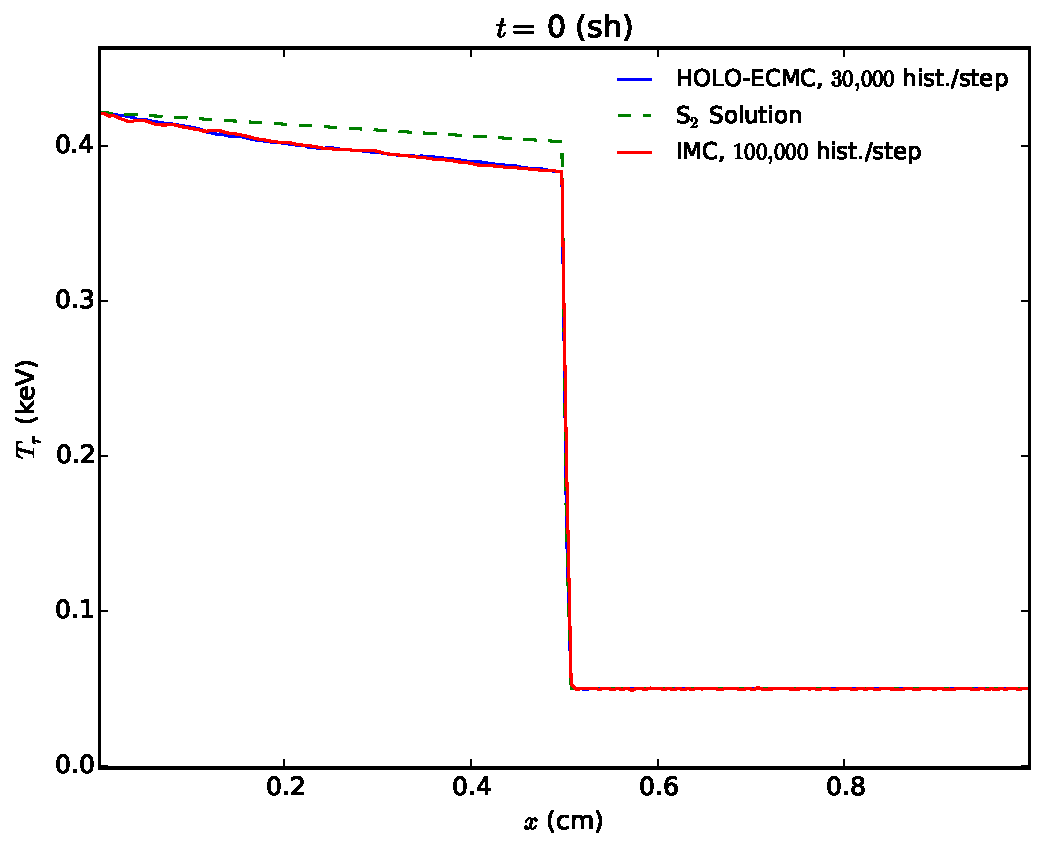
\includegraphics[width=0.5799\textwidth]{quick_compare.pdf}
\end{figure}

\end{frame}




\begin{frame}
    \frametitle{LO System}
    \begin{itemize}
        \item Taking moments of TE yields \colb{4 equations}, per cell $i$, e.g.
\begin{multline}\label{lo_tran}
    -2{\mu}_{i-1/2}^{n+1,+} \phi_{i-1/2}^{n+1,+} + \cur {\mu}_{L,i}^{n+1,+}
  \mom{\phi}_{L,i}^{n+1,+}
  +  \cur\mu_{R,i}^{n+1,+}
  \mom{\phi}_{R,i}^{n+1,+} +  \\ \left(\sigma_t^{n+1}+\frac{1}{c \Delta t} \right) h_i 
  \mom{\phi}_{L,i}^{n+1,+} -  \frac{\sigma_s h_i}{2} \left( \mom{\phi}_{L,i}^{n+1,+} +
  \mom\phi_{L,i}^{n+1,-}\right) \\ = \frac{h_i}{2} \mom{\sigma_a^{n+1} a c T^{n+1,4}}_{L,i} +
  \frac{h_i}{c\Delta t}\mom{\phi}_{L,i}^{n,+},
\end{multline}
        \item Cell unknowns: $\mom{\phi}_{L,i}^{+}$, $\mom{\phi}_{R,i}^{+}$,
        $\mom{\phi}_{L,i}^{-}$, $\mom{\phi}_{R,i}^{-}$, $T_L$, $T_R$

    \item Need \colb{angular} consistency terms  and spatial closure
        (LD)
    \end{itemize}

\end{frame}

\begin{frame}
    \frametitle{Solving LO System with Newton's Method}
    \begin{block}{}
    \begin{itemize}
        \item Linearization: $\displaystyle \u B(T^{n+1}) = \u B(T^*) + \left(T^{n+1} -
                T^*\right) \pderiv{\u B}{t}\bigg|_{t^*}$
        \vspace{-0.15in}
        \item Modified system
            \begin{gather*}
                \displaystyle \left[\B  D(\mu^\pm) - \sigma_a^*(1-f^*) \right]\underline
                \Phi^{n+1}  = f^* \u B(T^*) + \frac{ \underline \Phi^n}{c\Delta t} \\
                \boxed{\hat{ \B  D }\Phi^{n+1} = \underline Q}
            \end{gather*}
        \vspace{-0.07in}
        \begin{center}
         $\displaystyle f = \left( 1 + \sigma_a^*c \Delta t \frac{4aT^{*3}}{\rho
            c_v} \right)^{-1}$  \hspace{0.3in}
         $\displaystyle T_i^* = \frac{T^{*}_{L,i}+T^{*}_{R,i}}{2}$
     \end{center}
 \item Equation for $T^{n+1}$ based on linearization that is conservative
 \item Converge $T^{n+1}$ and $\mom{\phi}$ with Newton Iterations
     \begin{itemize}
 \item Spatial representation can result in negative temperatures
     \end{itemize}
 \end{itemize}
 \end{block}
\end{frame}

\setcounter{framenumber}{\value{finalframe}}
\end{document}
